\documentclass[12pt]{article}

\usepackage{graphicx}
\usepackage{float}
\usepackage{amsmath}
\usepackage{amssymb}
\usepackage{graphicx}
\usepackage[utf8]{inputenc}
\usepackage[spanish]{babel}
\usepackage{geometry}
\geometry{left=2cm,right=2cm,top=2cm,bottom=2cm}
\usepackage{listings}
\lstset{basicstyle=\ttfamily,
  showstringspaces=false,
  commentstyle=\color{red},
  keywordstyle=\color{blue}
}


\title{%
  Scan Conversion\\
  \large Tarea 03 \\
    \Large Computación Gráfica\\
     \large UNAM 2022-2}
\author{Gibran Zazueta Cruz \\
\small 03/marzo/2022}
\date{}

\begin{document}
\maketitle

\section{Introducción}

Se programa el algoritmo de scan conversion para rellenas las caras de un cuboide.
El objeto y estructura de la escena es la misma que se utilizó para la tarea 2.



\section{Estructura del código}

El programa tiene como base el código de la tarea 2.\\

EN cam projection se programa el scan conversion para rellenar el poligono

La función drawCubeFaces() recibe las coordenadas de cad una de las 6 caras del cubo. Llama a la funcion scanFillPoly para realizar el scan conversion siguiendo cada una de las aristas.

Después de la información de las aristas se ingrsan los puntos a dibujar a rasterPOints para que posteriromente sean dibujados por el canvas

En renderwindow se realizó una implementación de DDA co la función lide DDA

\section{Ejecutar el programa}
En la carpeta de build se puede ejecutar el programa con el archivo ScanConversion-Run. Desde la consola de comandos de linux:

\begin{lstlisting}[language=bash,title={bash}]
./ScanConversion-Run
\end{lstlisting}


En la carpeta principal está el código fuente. Para generar el ejecutable primero se genera el Makefile con

\begin{lstlisting}[language=bash,title={bash}]
 qmake ScanConversion.pro
\end{lstlisting}

Después se construye el proyecto con \textit{make}



\section{Instrucciones de uso}

Se agregan los botones FIll poly y Draw edeges para dibujar o borrar rellenado y bordes.

EL programa inicia solo dibujando bordes. Al precionar Fillpoly se rellenarán las caras del polígono. AL presionar una segunda vez se borraràn las caras. Draw Edges teine un comportamineto similar.

EL boton rotate cube hace rotar el cubo sobre su eje x, de manra constante
LOs botones perspectiva y ortografica cambian la proyeccion correspondiente


\section{Programa en ejecución}

\begin{figure}[H]
\centering
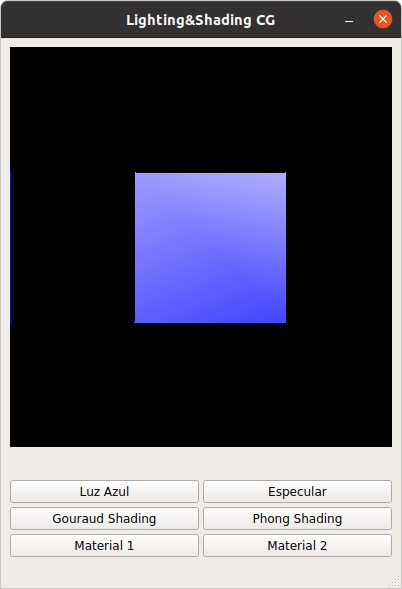
\includegraphics[scale=0.5]{images/ej1.png}
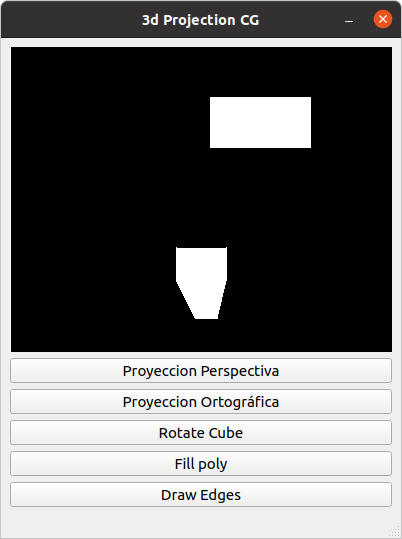
\includegraphics[scale=0.5]{images/ej2.png}
\caption{Proyección perspectiva y ortogonal de cámara 1 y 2}
\end{figure}

\begin{figure}[H]
\centering
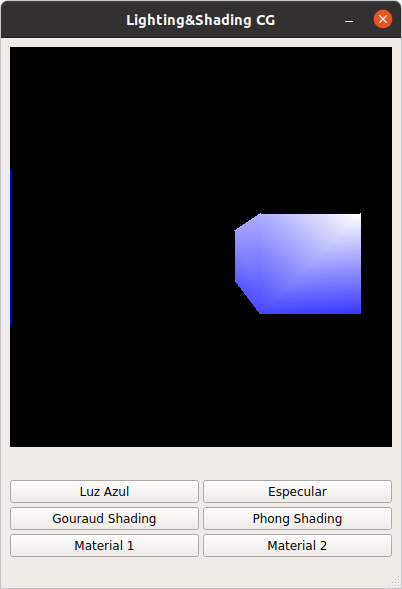
\includegraphics[scale=0.5]{images/ej3.png}
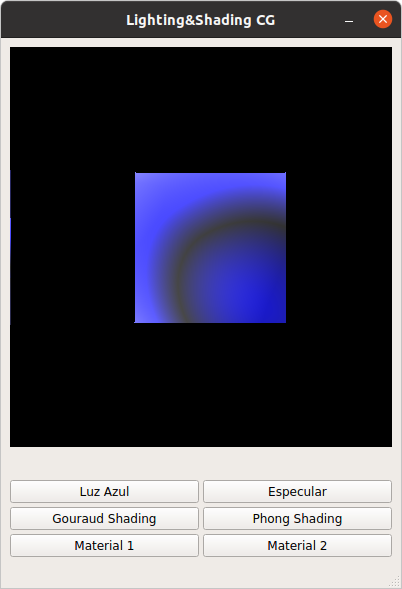
\includegraphics[scale=0.5]{images/ej4.png}
\caption{Proyección perspectiva y ortogonal después de rotar el cubo sobre X}
\end{figure}


\begin{thebibliography}{99}

\bibitem{uno} Collins, R. Lecture 12: Camera Projection. Penn State (http://www.cse.psu.edu/~rtc12/CSE486/lecture12.pdf)

\end{thebibliography}


\end{document}